\documentclass[border=3pt]{standalone}
% Preâmbulo compartilhado pelos diagramas TikZ da aula 8 de IHC (Design de IHC)
\usepackage[T1]{fontenc}
\usepackage[utf8]{inputenc}
\usepackage{lmodern}
\usepackage{amsmath}
\usepackage{xcolor}
\usepackage{tikz}
\usetikzlibrary{arrows.meta,angles,quotes,decorations.pathmorphing,decorations.pathreplacing,calc,
                positioning,shapes.geometric,shapes.misc,backgrounds,fit,
                math}

% Paleta (mesma dos SVGs originais)
% Paleta da disciplina de IHC: acento roxo (#755099), da capa do livro.
% (o nome "dblue" é mantido para não alterar todos os diagramas)
\definecolor{dblue}{HTML}{755099}
\definecolor{dorange}{HTML}{B3541E}
\definecolor{dgreen}{HTML}{4A7C59}
\definecolor{dred}{HTML}{9C4B4B}
\definecolor{dcream}{HTML}{F4F1EA}
\definecolor{dshade}{HTML}{DDD7C9}

% Função gaussiana (não normalizada por padrão de escala visual)
\pgfmathdeclarefunction{gauss}{3}{%
  \pgfmathparse{1/(#3*sqrt(2*pi))*exp(-((#1-#2)^2)/(2*#3^2))}%
}

% Estilos comuns (prefixo d... para não colidir com chaves internas do pgf)
\tikzset{
  >={Stealth[length=2mm]},
  dguide/.style={gray!55, dashed, line width=0.4pt},
  daxis/.style={gray!60, line width=0.7pt, ->},
  dbody/.style={fill=black!3, draw=black!80, line width=1pt},
  dacc/.style={draw=dblue, line width=1pt},
  dlbl/.style={black!55, font=\small},
  dsub/.style={black!45, font=\footnotesize},
  dstate/.style={circle, draw=black!80, fill=dcream, line width=1pt,
                 minimum size=17mm, font=\large, inner sep=1pt},
  dobs/.style={circle, draw=black!80, fill=dshade, line width=1pt,
               minimum size=14mm, font=\large, inner sep=1pt},
  dbox/.style={rounded corners=2pt, draw=black!80, fill=dcream, line width=1pt,
               align=center, inner sep=6pt},
  dop/.style={circle, draw=black!80, fill=white, line width=1pt,
              minimum size=6mm, inner sep=0pt, font=\small},
  dtrans/.style={->, dblue, line width=1pt},
  dmeas/.style={->, dorange, line width=1pt},
  dcurve/.style={line width=1pt, dblue},
  dcurveb/.style={line width=1.4pt, dorange},
}

\begin{document}
\hyphenpenalty=10000 \exhyphenpenalty=10000 \tolerance=9999 \emergencystretch=3em
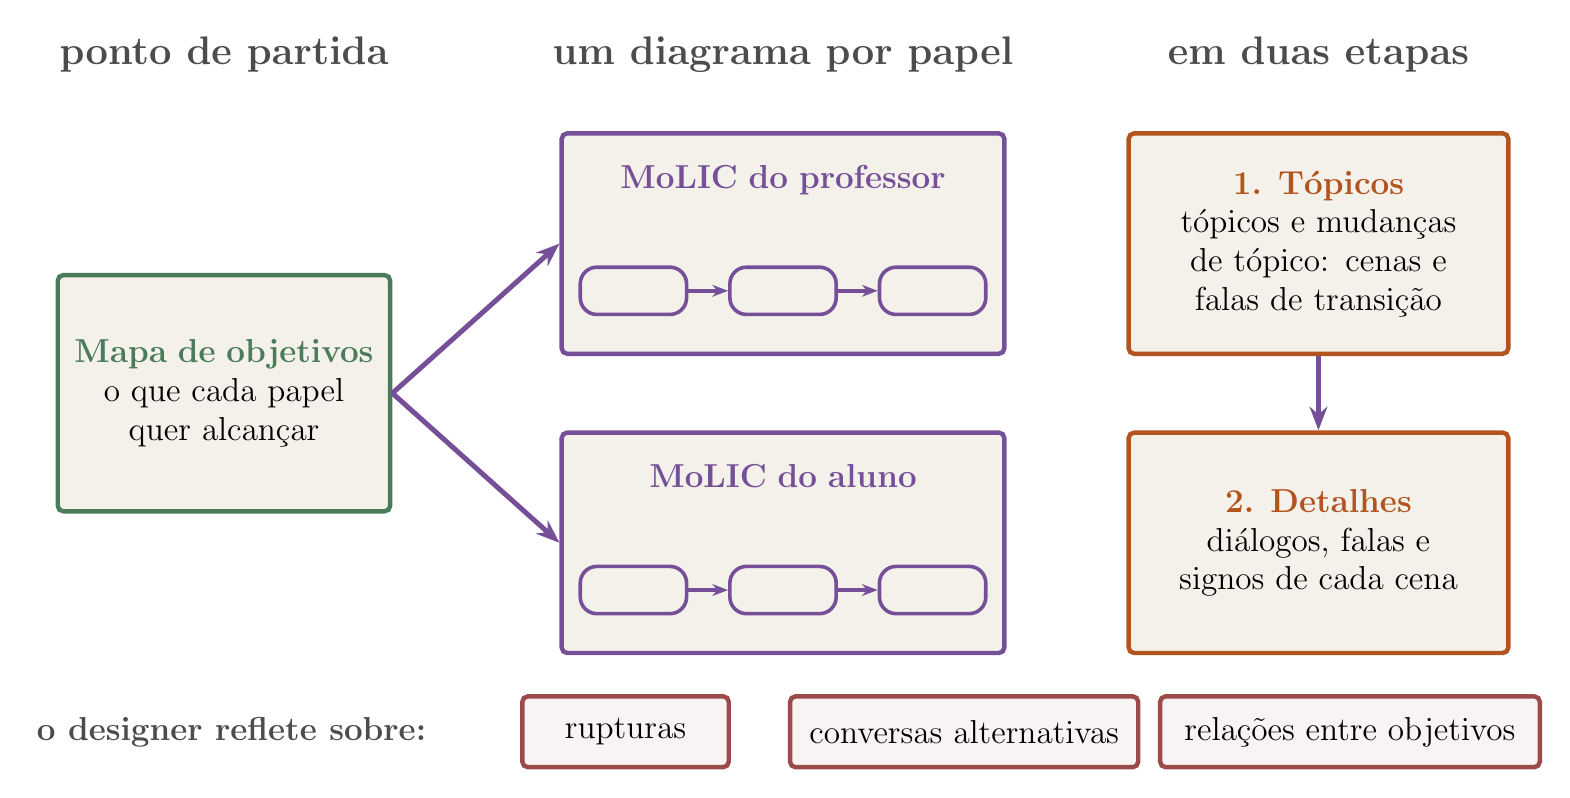
\begin{tikzpicture}[x=1cm,y=1cm]
\tikzset{c/.style={dbox, line width=1.6pt, font=\large}}
\node[font=\Large\bfseries, black!70] at (2.5,9.2) {ponto de partida};
\node[font=\Large\bfseries, black!70] at (9.6,9.2) {um diagrama por papel};
\node[font=\Large\bfseries, black!70] at (16.4,9.2) {em duas etapas};
\node[c, draw=dgreen, text width=3.8cm, minimum height=3.0cm] (mo) at (2.5,4.9) {\textbf{\textcolor{dgreen}{Mapa de objetivos}}\\ o que cada papel quer alcançar};
\node[c, draw=dblue, text width=5.2cm, minimum height=2.8cm] (p) at (9.6,6.8) {\textbf{\textcolor{dblue}{MoLIC do professor}}\\[34pt] \phantom{x}};
\node[c, draw=dblue, text width=5.2cm, minimum height=2.8cm] (a) at (9.6,3.0) {\textbf{\textcolor{dblue}{MoLIC do aluno}}\\[34pt] \phantom{x}};
\node[dbox, draw=dblue, rounded corners=6pt, line width=1.3pt, minimum width=1.35cm, minimum height=0.6cm, inner sep=1pt] (m96_0) at (7.699999999999999,6.2) {};
\node[dbox, draw=dblue, rounded corners=6pt, line width=1.3pt, minimum width=1.35cm, minimum height=0.6cm, inner sep=1pt] (m96_1) at (9.6,6.2) {};
\node[dbox, draw=dblue, rounded corners=6pt, line width=1.3pt, minimum width=1.35cm, minimum height=0.6cm, inner sep=1pt] (m96_2) at (11.5,6.2) {};
\draw[dblue, line width=1.3pt, -{Stealth[length=2mm]}] (m96_0.east) -- (m96_1.west);
\draw[dblue, line width=1.3pt, -{Stealth[length=2mm]}] (m96_1.east) -- (m96_2.west);\node[dbox, draw=dblue, rounded corners=6pt, line width=1.3pt, minimum width=1.35cm, minimum height=0.6cm, inner sep=1pt] (m96_0) at (7.699999999999999,2.4) {};
\node[dbox, draw=dblue, rounded corners=6pt, line width=1.3pt, minimum width=1.35cm, minimum height=0.6cm, inner sep=1pt] (m96_1) at (9.6,2.4) {};
\node[dbox, draw=dblue, rounded corners=6pt, line width=1.3pt, minimum width=1.35cm, minimum height=0.6cm, inner sep=1pt] (m96_2) at (11.5,2.4) {};
\draw[dblue, line width=1.3pt, -{Stealth[length=2mm]}] (m96_0.east) -- (m96_1.west);
\draw[dblue, line width=1.3pt, -{Stealth[length=2mm]}] (m96_1.east) -- (m96_2.west);
\draw[dtrans, line width=1.8pt, -{Stealth[length=3mm]}] (mo.east) -- (p.west);
\draw[dtrans, line width=1.8pt, -{Stealth[length=3mm]}] (mo.east) -- (a.west);
\node[c, draw=dorange, text width=4.4cm, minimum height=2.8cm] (e1) at (16.4,6.8) {\textbf{\textcolor{dorange}{1. Tópicos}}\\ tópicos e mudanças de tópico: cenas e falas de transição};
\node[c, draw=dorange, text width=4.4cm, minimum height=2.8cm] (e2) at (16.4,3.0) {\textbf{\textcolor{dorange}{2. Detalhes}}\\ diálogos, falas e signos de cada cena};
\draw[dtrans, line width=1.8pt, -{Stealth[length=3mm]}] (e1.south) -- (e2.north);
\node[font=\large\bfseries, black!70, anchor=west] at (0.0,0.6) {o designer reflete sobre:};
\node[c, draw=dred, fill=dred!6, text width=2.2cm, minimum height=0.9cm] at (7.6,0.6) {rupturas};
\node[c, draw=dred, fill=dred!6, text width=4.0cm, minimum height=0.9cm] at (11.9,0.6) {conversas alternativas};
\node[c, draw=dred, fill=dred!6, text width=4.4cm, minimum height=0.9cm] at (16.8,0.6) {relações entre objetivos};
\end{tikzpicture}
\end{document}
